\chapter{Arquitetura de Software}
\label{sec-arquitetura}
\vspace{-1cm}

A Figura~\ref{figura-arquitetura} mostra a arquitetura do sistema \emph{\imprimirtitulo}.

\begin{figure}[h]
	\centering
	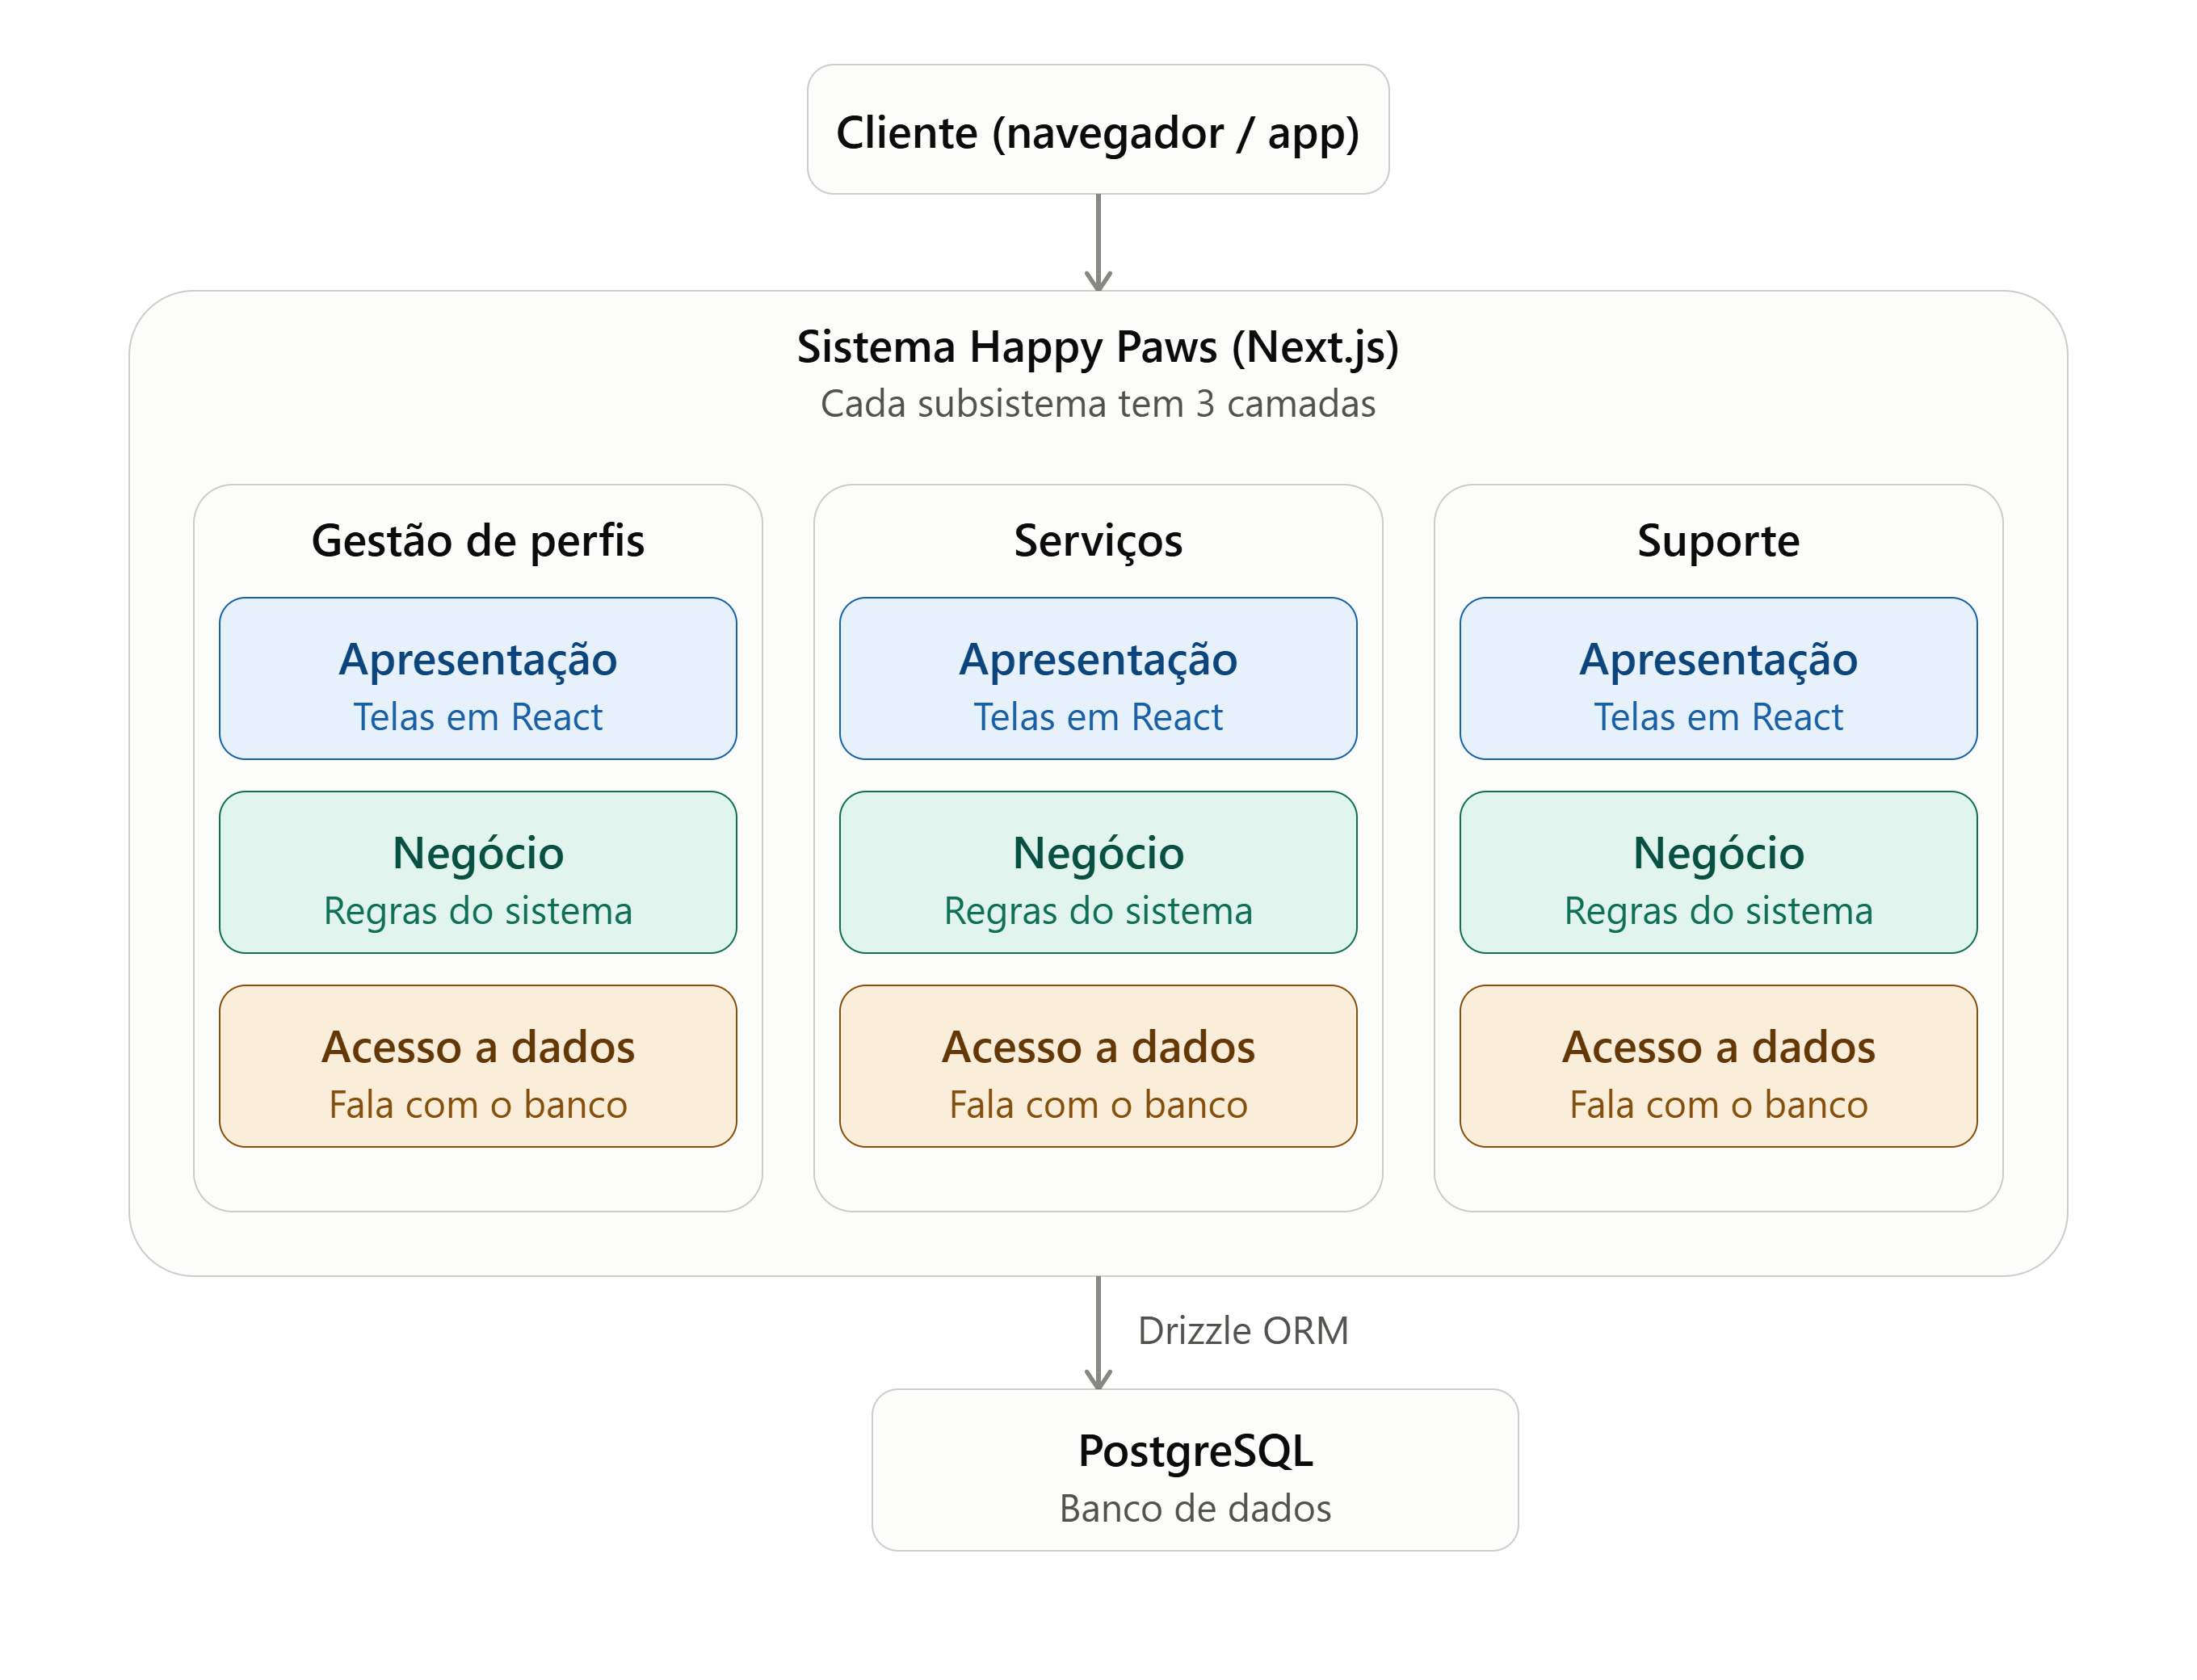
\includegraphics[width=1\textwidth]{figuras/arquitetura_camadas_happy_paws.png}
	\caption{Arquitetura do sistema.}
	\label{figura-arquitetura}
\end{figure}

O sistema Happy Paws usa uma Arquitetura em Camadas~\cite{fowler:book02}. Essa arquitetura é usada nos três subsistemas do sistema: Gestão de Perfis, Serviços e Suporte, como mostra a Figura~\ref{figura-arquitetura}. As camadas são: Apresentação, Negócio e Acesso a Dados.

A camada de Apresentação mostra as telas do sistema e recebe as ações do usuário. Ela é feita com componentes React do Next.js, usando a biblioteca shadcn/ui e o Tailwind CSS para o visual.

A camada de Negócio tem as regras do sistema. Por exemplo, não deixar cadastrar dois usuários com o mesmo CPF, ou não deixar um passeador levar mais cães do que o limite dele. Essa camada é feita com \emph{Server Actions} do Next.js. Ela fica entre a camada de Apresentação e a camada de Acesso a Dados.

A camada de Acesso a Dados fala com o banco de dados. Ela guarda, busca, atualiza e apaga as informações do sistema no PostgreSQL, usando o Drizzle ORM.